\section{Programstruktur}
Baseret på de førnævnte krav blev designfasen påbegyndt. Målet er at forsimple opgaven for brugeren så meget som overhovedet muligt, da det ikke vil kunne forventes at denne person kender noget til det bagvedliggende system.
Tilsvarende ønskes der en simpel og generel anvendelse af programmets services fra de højere lag nær chat-klienten, hvorimod de mere administrative og praktiske funktionaliteter skal håndteres længere nede i systemet.

\begin{figure}[h!]
\centering
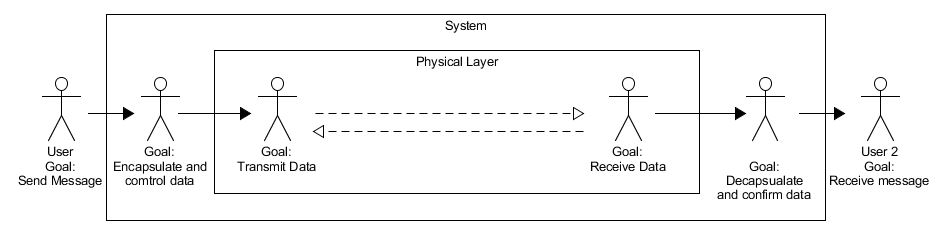
\includegraphics[scale=0.5]{Billeder/ProgramOpbygning1.JPG}
\caption{Systemopbygning - første udkast}
\label{fig:Blokdiagram}
\end{figure}

Figur \ref{fig:Blokdiagram} viser første udkast til programmets struktur i grove træk. Afsenderen modtager data fra brugeren, og indkapsler dette i et format modtageren er i stand til at bearbejde. Herfra tager det næste lag sig ad den reelle transmission og afkodning af informationen. Dette lag er upålideligt, så modtageren skal tilsvarende her validere indholdet og rækkefølgen af informationen, for at kunne sikre en korrekt transmission.

I og med at den ønskede applikation er et chat-program, er det af høj prioritet, at den logiske forbindelse mellem de to brugere er pålidelig. Dette indebærer, at det som afsenderen skriver, skal være præcis det samme, som modtageren læser. Systemet vil derfor tage udgangspunkt i TCP/IP, da denne protokol vigtigst af alt tilbyder en pålidelig overførsel af data. 


\subsection{Designklassediagram}
Næste step i arbejdsprocessen bliver at opsætte et klassediagram, hvori dataoverførelsen skal nedbrydes i flere klasser med hver sit ansvarsområde, og funktionaliteter der passer hertil. Normalt kræver det, for at kunne udarbejde et designklassediagram, at der inden er udarbejdet en domænemodel, baseret på objekter fra den virkelige verden, men da dette projekt er et rent software problem, vil dette step ikke tilføre nogen værdi til projektet. 

\begin{figure}[h]
\centering
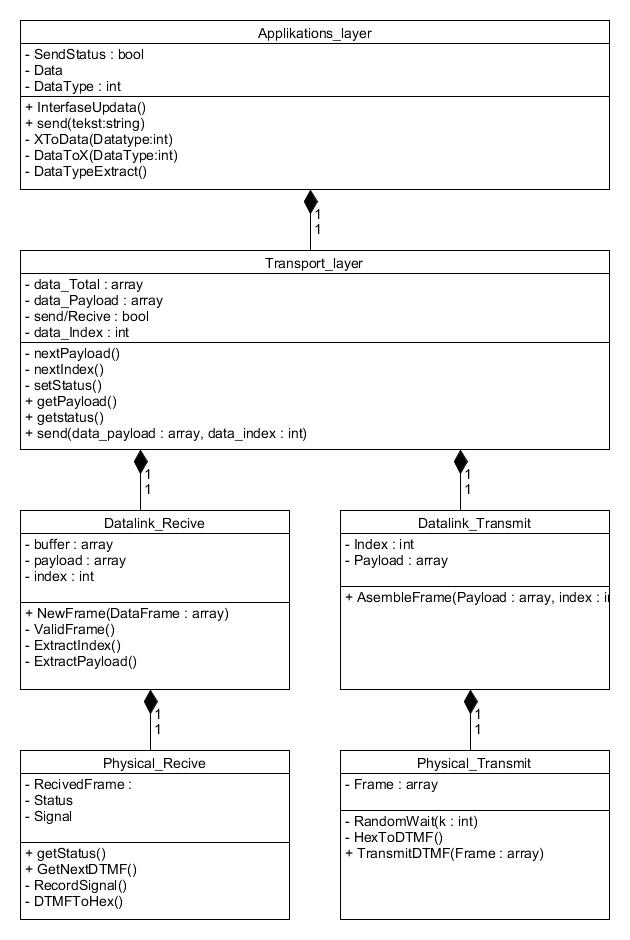
\includegraphics[scale=0.45]{Billeder/Klassediagram_v1.jpg}
\caption{Her vises designklassediagram}
\label{fig:Klassediagram_v1}
\end{figure}

Det er ønsket at opnå en lagdelt struktur af programmet, da dette giver den fordel, at ændringer på ét lag ikke påvirker resten af programmets virkemåde, sålænge at inputtet og outputtet forbliver af samme format. Programmet er inddelt i fire lag:  Applikationslaget, transportlaget, datalinklaget og det fysiske lag. Heraf er datalinklaget og det fysiske lag opdelt i en afsender- og modtagerdel. Dette ses af figur \ref{fig:Klassediagram_v1}. Denne struktur er inspireret af internettets syvlagsmodel, men da der ikke er behov for at route datapakker, vil der ikke være behov for netværkslaget.

For at anvende den service programmet tilbyder, er det nok at inkludere klassen "Application Layer" og oprette et objekt heraf. Dette kan lade sig gøre, da de underliggende objekter håndteres af applikationslaget. Applikationslaget kan derfor betragtes som værende systemets "controller".

Det opstillede designklassediagram vil blive anvendt som en retningslinje for programmets opbygning, men da det i dette stadie af projektet kan være svært at tage højde for alt, vil det ikke være utænkeligt der måtte forkomme ændringer her i.


\subsection{Ansvarsfordeling og grænseflader}
For at sikre en "high cohesion", nedbrydes programmet til et sæt af veldefinerede ansvarsområder og grænseflader mellem programmets forskellige lag. På den måde vil flere mennesker kunne arbejde på samme projekt uafhængig af hinanden.  

\textbf{Det fysiske lag} har ansvaret for alt hvad der kræves for succesfuldt at afsende DTMF-toner og modtage dem igen på den anden side. Dette betyder, at det fysiske lag på afsenderens side kan forvente at modtage et array af bits (bools) som skal transmitteres, og forventes at returnere et array af bits på modtagersiden. Det fysiske lag må under intet tidspunkt i denne proces forholde sig til indholdet af denne besked, men må gerne tilføje ekstra data, så længe at det tilsvarende fjernes igen, inden det når næste lag.

\textbf{Datalinklaget} har ansvaret for indpakning og udpakning af den mængde informationer, som anvendes på laget over. Disse oplysninger skal på afsendersiden pakkes ind i et array af bits kaldet en frame, som det fysiske lag kan sende og modtage. På modtagersiden vil der modtages et array, som skal  konverteres tilbage til de oplysninger, der oprindeligt blev sendt på afsendersiden og returneres til transportlaget. 
Datalinklaget har yderligere ansvaret for at sikre, at korrupte pakker eller pakker med forkert adresse aldrig når de øvre lag.

\textbf{Transportlaget} har ansvaret for, at alle pakker modtaget fra det øverste lag når frem, og i korrekt rækkefølge. Mellem transportlaget og applikationslaget udveksles arrays af bits. Transportlaget må, ligesom det fysiske lag, ikke forholde sig til indholdet af disse arrays. I grænsefladen mellem transportlaget og datalinklaget, vil der blive overført en datapakke, sammen med administrative oplysninger som modtageradresse, beskedtype og indeksering. 

\textbf{Applikationslaget} har ansvaret at konvertere beskeder fra hvad brugeren ønsker at sende, til et array af bools, og tilbage igen. Programmet kan derfor understøtte flere dataformater, ved blot at tilføje funktionalitet på dette lag. 
Dette lag har ansvaret for at opdele beskeden i pakker som kan håndteres af transportlaget, og på tilsvarende vis samle pakker modtaget fra transportlaget til den afsendte besked. På dette lag kan det antages at pakker modtages i korrekt rækkefølge, og uden fejl. 